\hypertarget{freud}{%
\section{Freud!}\label{freud}}

\begin{figure}[!ht]
  \begin{adjustwidth}{-\oddsidemargin-1in}{-\rightmargin}
    \centering
    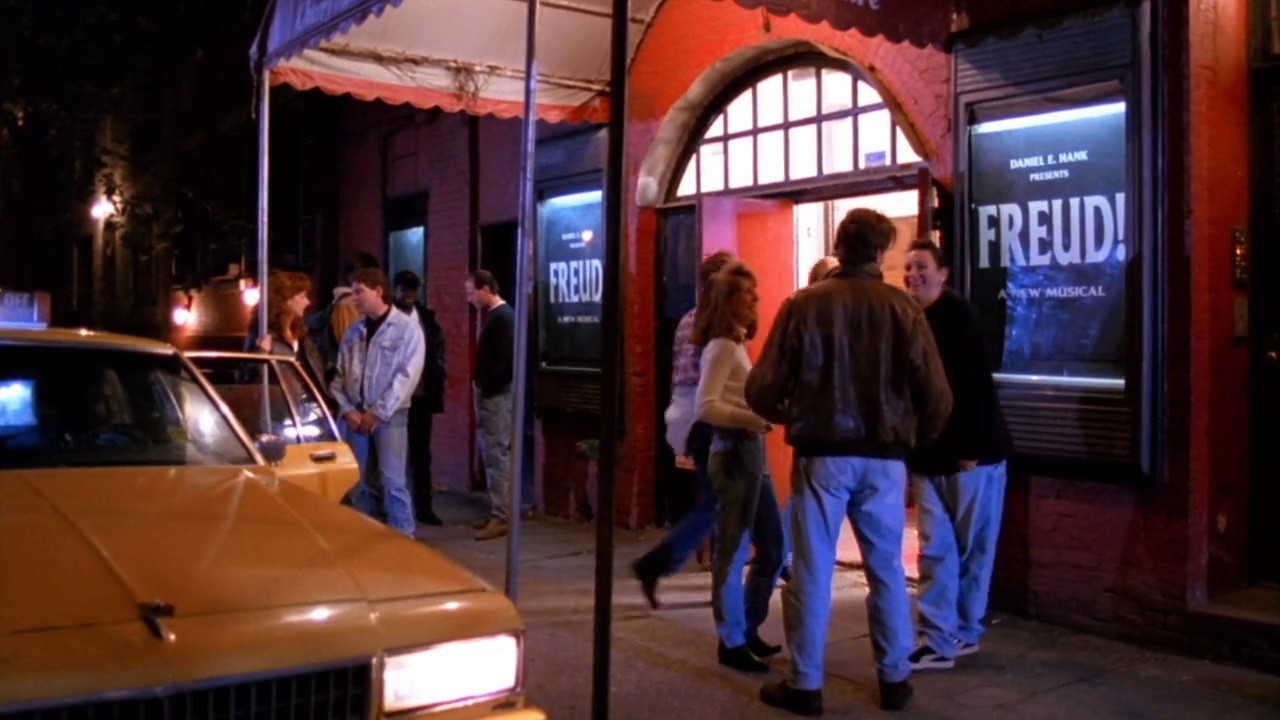
\includegraphics[trim={0 7cm 0 3cm,}, clip, width=\paperwidth]{./S01/img/6/freud.png}
    % \caption{Freud\label{fig:freud}}
  \end{adjustwidth}
\end{figure}

Joey é o protagonista do musical \emph{Freud!}, atuando como
\emph{Sigmund Freud} (1856), considerado o Pai da Psicanálise. No
musical, Joey canta uma música sobre um assunto abordado no livro de
Freud chamado \emph{The Psychical Consequences of the Anatomic
Distinction Between the Sexes} (1925), onde ele explica algo que ficou
conhecido como `Penis Envy' (Inveja do pênis).\footnote{\sloppy Freud and penis envy - a failure of courage? - The British Psychological Society (Inglês). \url{https://thepsychologist.bps.org.uk/volume-31/june-2018/freud-and-penis-envy-failure-courage}}

\begin{quote}
All you want is a dinkle
\end{quote}

\begin{quote}
What you envy's a schwang
\end{quote}

\begin{quote}
A thing through which you can tinkle
\end{quote}

\begin{quote}
To play with or simply let hang
\end{quote}

Na letra, \emph{dinkle} e \emph{schwang} são metáforas para pênis.

\hypertarget{richard-leakey}{%
\section{Richard Leakey}\label{richard-leakey}}

\begin{figure}[!ht]
  \begin{adjustwidth}{-\oddsidemargin-1in}{-\rightmargin}
    \centering
    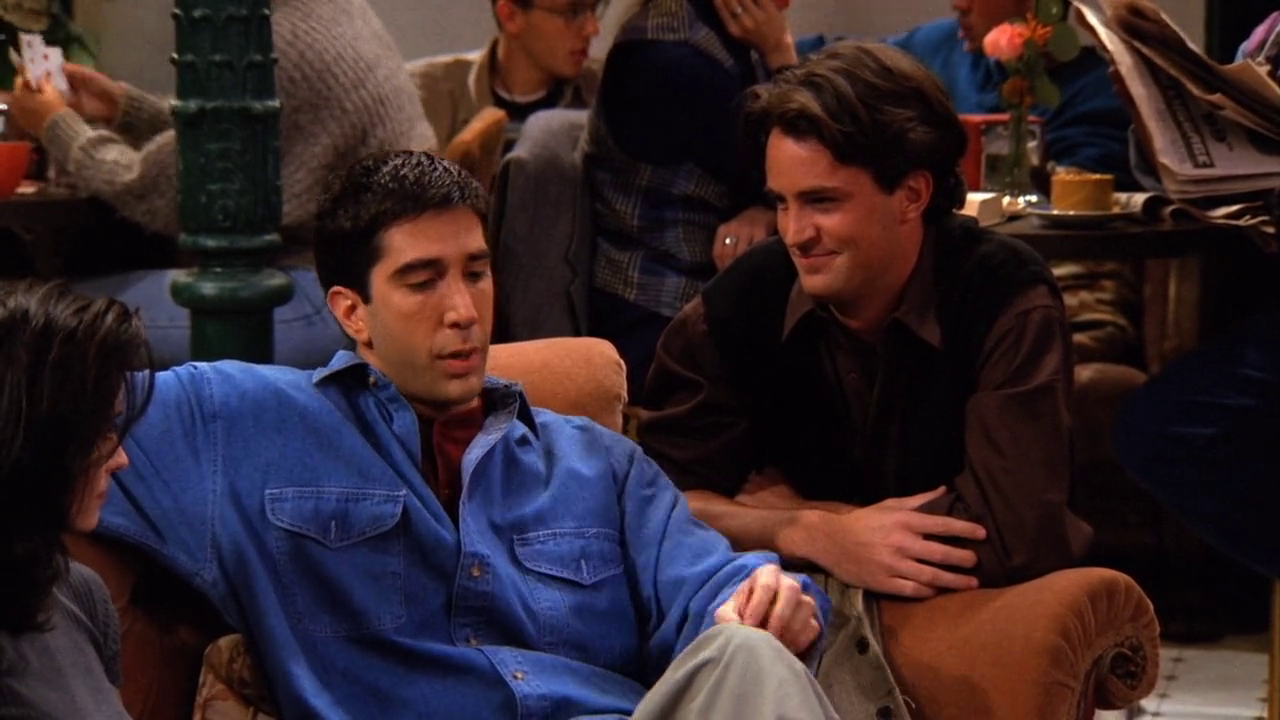
\includegraphics[trim={0 7cm 0 2cm,}, clip, width=\paperwidth]{./S01/img/6/richard-leakey.png}
    % \caption{Richard Leakey\label{fig:richard-leakey}}
  \end{adjustwidth}
\end{figure}

\begin{tcolorbox}[enhanced,center upper,
    drop fuzzy shadow southeast, boxrule=0.3pt,
    lower separated=false, breakable,
    colframe=black!30!dialogoBorder,colback=white]
\begin{minipage}[c]{0.16\linewidth}
  \raisebox{\dimexpr-\height+\ht\strutbox\relax}{
    \centering 
\includegraphics[width=1.4cm]{./assets/img/ross.png}
  }
   & \centering \scriptsize{Ross}
\end{minipage}
\hfill
\begin{minipage}[c]{0.8\linewidth}
  \textbf{- All right. There's a theory put forth by Richard Leakey...}\\
  - Certo. Há uma teoria de Richard Leakey...
\end{minipage}
\end{tcolorbox}

Enquanto discutem a relação de Chandler com Aurora, Ross tenta explicar
uma teoria de \emph{Richard Leakey} (1944), um antropólogo queniano. Uma
das suas mais importantes descobertas foi um esqueleto quase completo de
1,6 milhão de anos.\footnote{\sloppy Richard Leakey - Site oficial. \url{http://www.leakey.com/bios/richard-leakey}}

\begin{figure}
  \centering
  \begin{tikzpicture}
    \node [inner sep=0pt] at (0,0) {
      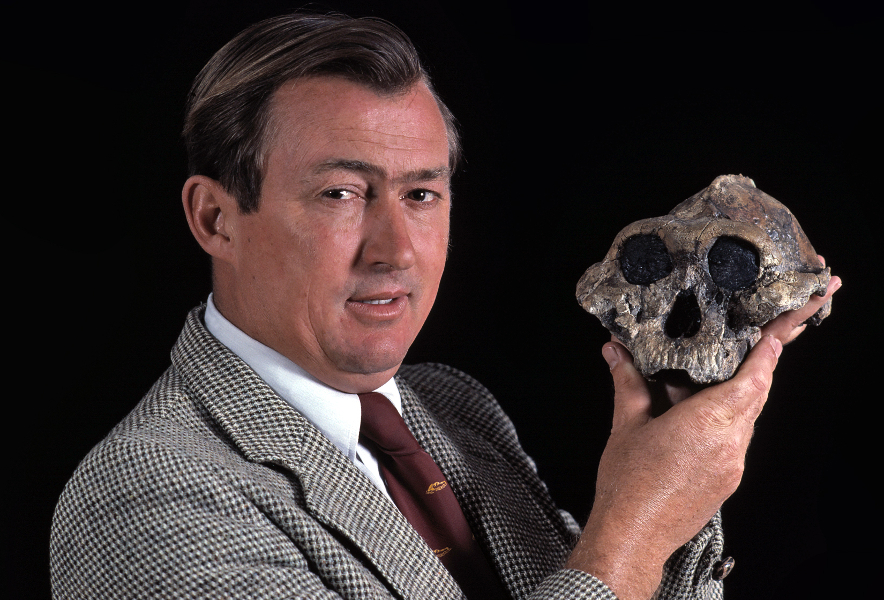
\includegraphics[width=0.6\textwidth,keepaspectratio]{./S01/img/6/richard-leakey-with-fossil.jpg}
    };
    \draw [white, rounded corners=\ClipSep, line width=\ClipSep]
    (current bounding box.north west) --
    (current bounding box.north east) --
    (current bounding box.south east) --
    (current bounding box.south west) -- cycle
    ;
    \end{tikzpicture}
    \caption{Richard Leakey with fossil\label{fig:richard-leakey-with-fossil}}
\end{figure}

\hypertarget{raggedy-ann}{%
\section{Raggedy Ann}\label{raggedy-ann}}

\begin{figure}[!ht]
  \begin{adjustwidth}{-\oddsidemargin-1in}{-\rightmargin}
    \centering
    
\includegraphics[trim={0 6cm 0 2cm,}, clip, width=\paperwidth]{./S01/img/6/raggedy-ann.png}
    % \caption{Raggedy Ann\label{fig:raggedy-ann}}
  \end{adjustwidth}
\end{figure}

\begin{tcolorbox}[enhanced,center upper,
    drop fuzzy shadow southeast, boxrule=0.3pt,
    lower separated=false, breakable,
    colframe=black!30!dialogoBorder,colback=white]
\begin{minipage}[c]{0.16\linewidth}
  \raisebox{\dimexpr-\height+\ht\strutbox\relax}{
    \centering 
\includegraphics[width=1.4cm]{./assets/img/ross.png}
  }
   & \centering \scriptsize{Ross}
\end{minipage}
\hfill
\begin{minipage}[c]{0.8\linewidth}
  \textbf{- When we were kids, yours was the only Raggedy Ann doll that wasn't raggedy.}\\
  - Quando criança, sua Raggedy Ann era a única boneca intacta.
\end{minipage}
\end{tcolorbox}

\saveparinfos
\noindent
\begin{minipage}[c]{0.5\textwidth}\useparinfo

Enquanto discutem como Monica é organizada, Ross menciona a boneca
\emph{Raggedy Ann}, personagem de um livro criada por \emph{Johnny
Gruelle} (1880-1938), que mais tarde se tornaria brinquedo. A ideia é
que a boneca parecesse velha e desgastada, daí o nome \emph{Raggedy},
que significa esfarrapada.\footnote{\sloppy Livro Raggedy Ann Stories - Projeto Gutemberg (Inglês). \url{https://www.gutenberg.org/ebooks/18190}}

\end{minipage}\hfill
\begin{minipage}[c]{0.5\textwidth}

\begin{figure}
  \centering
  \begin{tikzpicture}
    \node [inner sep=0pt] at (0,0) {
      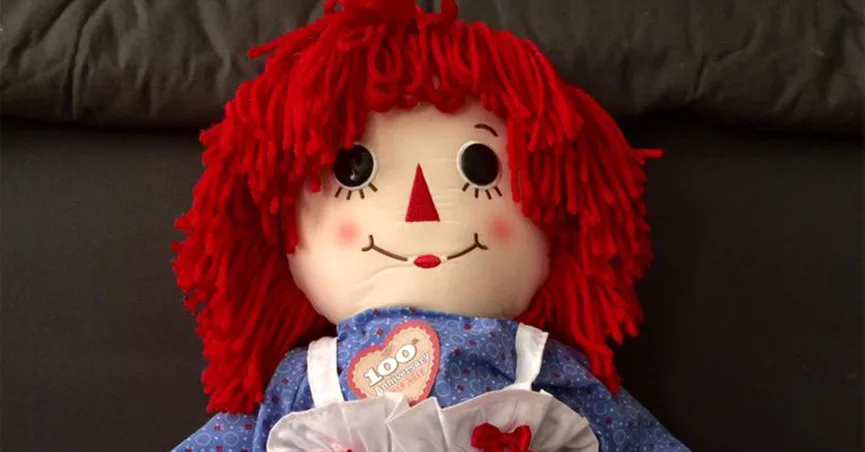
\includegraphics[width=0.8\textwidth,keepaspectratio]{./S01/img/6/raggedy-ann-doll.png}
    };
    \draw [white, rounded corners=\ClipSep, line width=\ClipSep]
    (current bounding box.north west) --
    (current bounding box.north east) --
    (current bounding box.south east) --
    (current bounding box.south west) -- cycle
    ;
    \end{tikzpicture}
    \caption{Raggedy Ann doll\label{fig:raggedy-ann-doll}}
\end{figure}

\end{minipage}

\hypertarget{al-pacino}{%
\section{Al Pacino}\label{al-pacino}}

\begin{figure}[!ht]
  \begin{adjustwidth}{-\oddsidemargin-1in}{-\rightmargin}
    \centering
    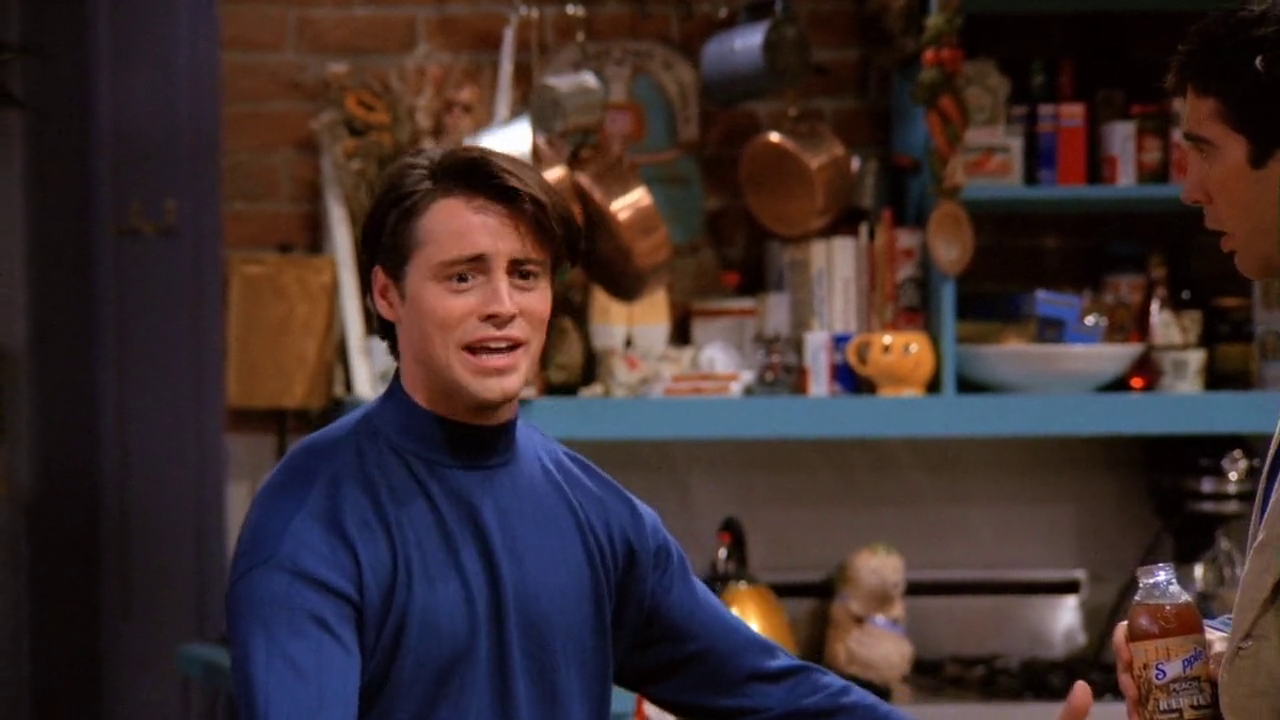
\includegraphics[trim={0 4cm 0 4cm,}, clip, width=\paperwidth]{./S01/img/6/al-pacino.png}
    % \caption{Al Pacino\label{fig:al-pacino}}
  \end{adjustwidth}
\end{figure}

\begin{tcolorbox}[enhanced,center upper,
    drop fuzzy shadow southeast, boxrule=0.3pt,
    lower separated=false, breakable,
    colframe=black!30!dialogoBorder,colback=white]
\begin{minipage}[c]{0.16\linewidth}
  \raisebox{\dimexpr-\height+\ht\strutbox\relax}{
    \centering 
\includegraphics[width=1.4cm]{./assets/img/joey.png}
  }
   & \centering \scriptsize{Joey}
\end{minipage}
\hfill
\begin{minipage}[c]{0.8\linewidth}
  \textbf{- My agent has just gotten me a job in the new Al Pacino movie!}\\
  - Minha agente arranjou um papel no novo filme de Al Pacino!
\end{minipage}
\end{tcolorbox}

Após conversar com sua agente, Joey dá a notícia que estará no novo
filme de \emph{Al Pacino} (1940), ator, diretor e produtor americano de
origem italiana. Joey ainda faz referências a dois filmes protagonizados
por Al Pacino:

\saveparinfos
\noindent
\begin{minipage}[c]{0.5\textwidth}\useparinfo

\begin{quote}
I'm out of order? You're out of order! This whole courtroom's out of
order!
\end{quote}

Trecho do filme \emph{\ldots And Justice for All} (1979), conhecido no
Brasil como \emph{Justiça para Todos}.\footnote{\sloppy …And Justice for All - IMDB. \url{https://www.imdb.com/title/tt0078718/?ref_=nv_sr_srsg_0}}
\footnote{\sloppy Citação de …And Justice for All - Shmoop. \url{https://www.shmoop.com/quotes/whole-courts-out-of-order.html}}

\end{minipage}\hfill
\begin{minipage}[c]{0.5\textwidth}

\begin{figure}
  \centering
  \begin{tikzpicture}
    \node [inner sep=0pt] at (0,0) {
      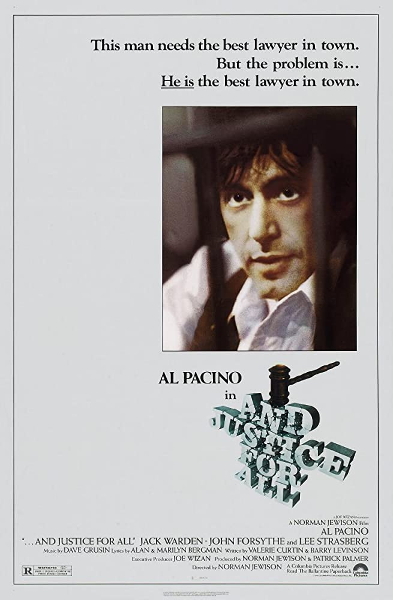
\includegraphics[width=0.6\textwidth,keepaspectratio]{./S01/img/6/and-justice-for-all-poster.jpg}
    };
    \draw [white, rounded corners=\ClipSep, line width=\ClipSep]
    (current bounding box.north west) --
    (current bounding box.north east) --
    (current bounding box.south east) --
    (current bounding box.south west) -- cycle
    ;
    \end{tikzpicture}
    \caption{…And Justice for All\label{fig:and-justice-for-all}}
\end{figure}

\end{minipage}

\saveparinfos
\noindent
\begin{minipage}[c]{0.5\textwidth}\useparinfo

E:

\begin{quote}
Just when I thought I was out, they pull me back in!
\end{quote}

Trecho do filme \emph{The Godfather: Part III} (1990), conhecido no
Brasil como \emph{O Poderoso Chefão III}.\footnote{\sloppy The Godfather: Part III - IMDB. \url{https://www.imdb.com/title/tt0099674/?ref_=nv_sr_srsg_3}}
\footnote{\sloppy Citação de The Godfather: Part III - Shmoop. \url{https://www.shmoop.com/quotes/just-when-i-thought-i-was-out.html}}

\end{minipage}\hfill
\begin{minipage}[c]{0.5\textwidth}

\begin{figure}
  \centering
  \begin{tikzpicture}
    \node [inner sep=0pt] at (0,0) {
      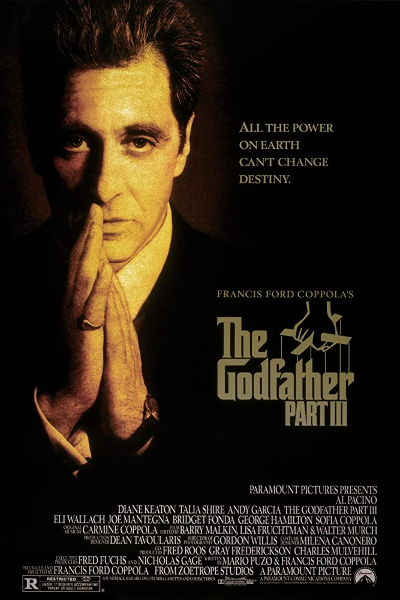
\includegraphics[width=0.6\textwidth,keepaspectratio]{./S01/img/6/the-godfather-iii-poster.jpg}
    };
    \draw [white, rounded corners=\ClipSep, line width=\ClipSep]
    (current bounding box.north west) --
    (current bounding box.north east) --
    (current bounding box.south east) --
    (current bounding box.south west) -- cycle
    ;
    \end{tikzpicture}
    \caption{The Godfather: Part III\label{fig:the-godfather-part-iii}}
\end{figure}

\end{minipage}

\hypertarget{its-a-wonderful-life}{%
\section{It's a Wonderful Life}\label{its-a-wonderful-life}}

\begin{figure}[!ht]
  \begin{adjustwidth}{-\oddsidemargin-1in}{-\rightmargin}
    \centering
    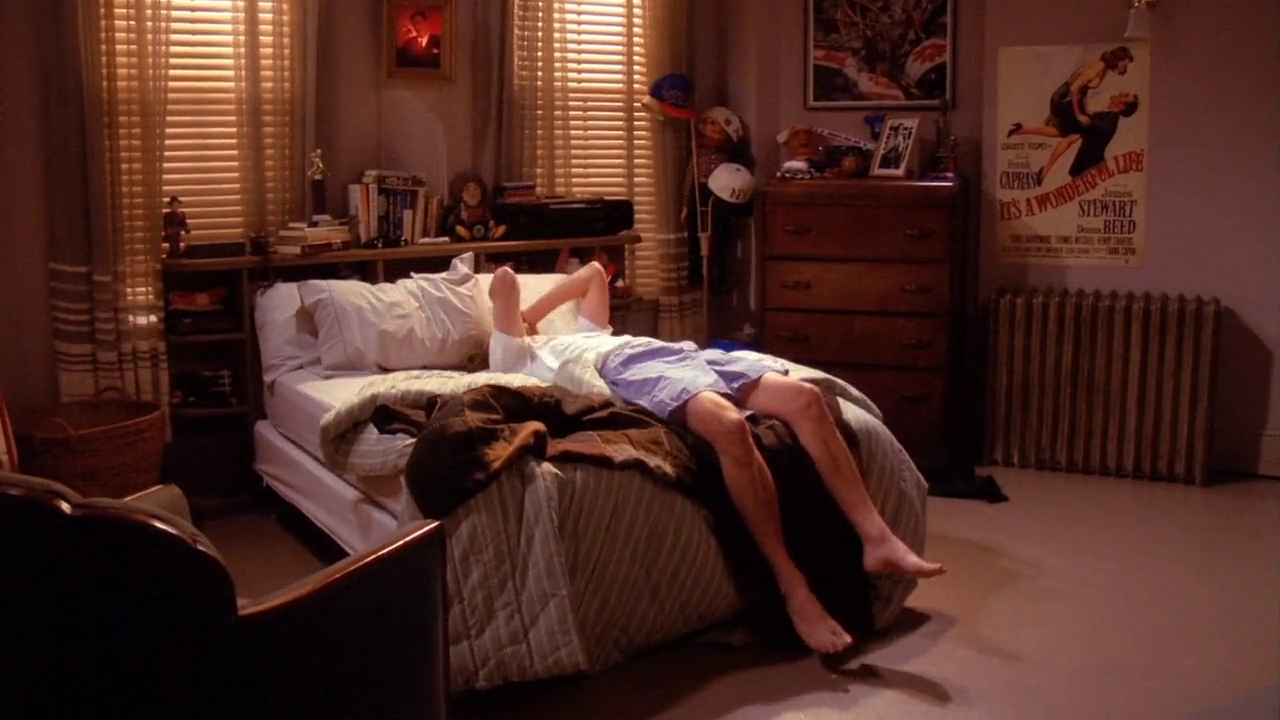
\includegraphics[trim={0 9cm 0 1cm,}, clip, width=\paperwidth]{./S01/img/6/its-a-wonderful-life.png}
    % \caption{It’s a Wonderful Life\label{fig:it-s-a-wonderful-life}}
  \end{adjustwidth}
\end{figure}

\saveparinfos
\noindent
\begin{minipage}[c]{0.5\textwidth}\useparinfo

Após termino do namoro com Aurora, é possível ver no quarto de Chandler
um poster do filme \emph{It's a Wonderful Life} (1946), filme
norte-americano de drama e fantasia. No Brasil, ficou conhecido como
\emph{A Felicidade Não se Compra}. É um dos filmes que Monica sugere a
Phoebe no episódio
\textbf{\textcolor{primarycolor}{S02E20 - The One Where Old Yeller Dies}}.\footnote{\sloppy It’s a Wonderful Life - IMDB. \url{https://www.imdb.com/title/tt0038650/}}

\end{minipage}\hfill
\begin{minipage}[c]{0.5\textwidth}

\begin{figure}
  \centering
  \begin{tikzpicture}
    \node [inner sep=0pt] at (0,0) {
      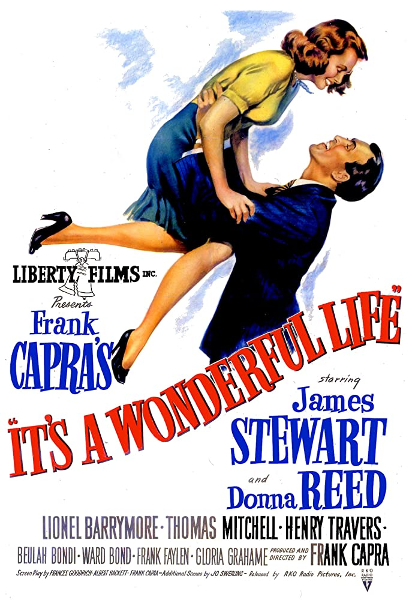
\includegraphics[width=0.6\textwidth,keepaspectratio]{./S01/img/6/its-a-wonderful-life-poster.jpg}
    };
    \draw [white, rounded corners=\ClipSep, line width=\ClipSep]
    (current bounding box.north west) --
    (current bounding box.north east) --
    (current bounding box.south east) --
    (current bounding box.south west) -- cycle
    ;
    \end{tikzpicture}
    \caption{It’s a Wonderful Life poster\label{fig:it-s-a-wonderful-life-poster}}
\end{figure}

\end{minipage}
